\section{System description}
\label{sec:sys}

This section will present a detailed description of our \ac{LTR} system.
Our system was designed to work by using 3D lidar scans as a primary mean of localization, also using \ac{IMU} and wheel odometry as input.
The main components of the framework are shown in~\autoref{fig:ltr_flow}.
As the \ac{ICP} algorithm is the foundation of this algorithm, our implementation of the \ac{ICP} algorithm is detailed first.
Next, the teach phase is described, explaining how the reference trajectory and map are logged.
Subsequently, the repeat phase is described, when the robot localizes within the map a simple controller allows computing commands that allow to repeat the reference trajectory.
Finally, the hardware used to deploy the \ac{LTR} system, including the \ac{UGV}, sensing and computing hardware is described.

\begin{figure} [h!]
	\centering
	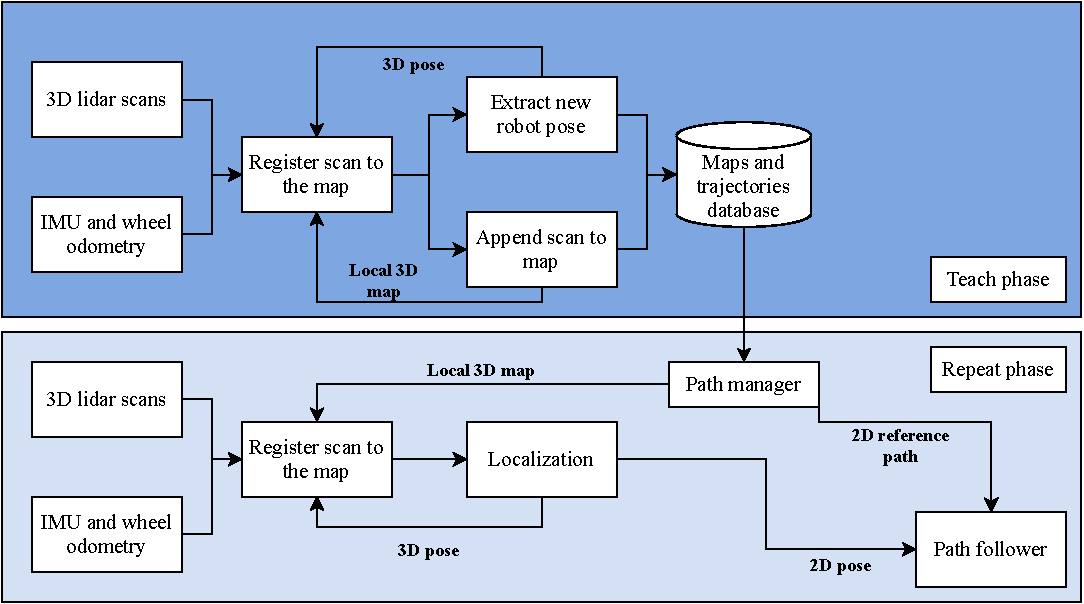
\includegraphics[height=2.8in]{figs/LTR_flowchart.pdf}
	\caption{Flowchart for LTR}
	\label{fig:ltr_flow}
\end{figure}

Various coordinate frames need to be defined for the \ac{LTR} framework to work, all of which are illustrated in~\autoref{fig:ltr_frames}.
First, a map frame $\mapf$ is defined representing the world in which the robot is navigating.
Second, a robot frame $\robotf$ is defined with its origin at the base of the robot chassis and the $x$-axis parallel to the longitudinal direction and the $y$-axis parallel to the lateral direction of the vehicle.
%The rigid transform \transform{\robotf}{\odomf} is updated at the rate of the \ac{IMU} and wheel odometry and used as a prior for the \ac{ICP} algorithm.
Thirdly, a lidar frame $\lidarf$ is defined at the origin of the lidar sensor.
The rigid transform from the robot frame to the lidar frame \transform{\robotf}{\lidarf} is assumed to be constant and found through system calibration.
Reading point clouds $\readpc$ are originally observed in the lidar frame $\lidarf$ and reference point clouds are expressed in the map frame $\mapf$.
The transform between $\robotf$ and $\mapf$ \transform{\robotf}{\mapf} is updated via the \ac{ICP} algorithm and is used as odometry for the robot.
Lastly, for path following algorithm, a Frenet-Serret frame $\pathf$ is defined directly on the path.
\todo{define 3d and 2d pose components}

%% TODO : Replace with our version of the figure
\begin{figure} [htpb]
	\centering
	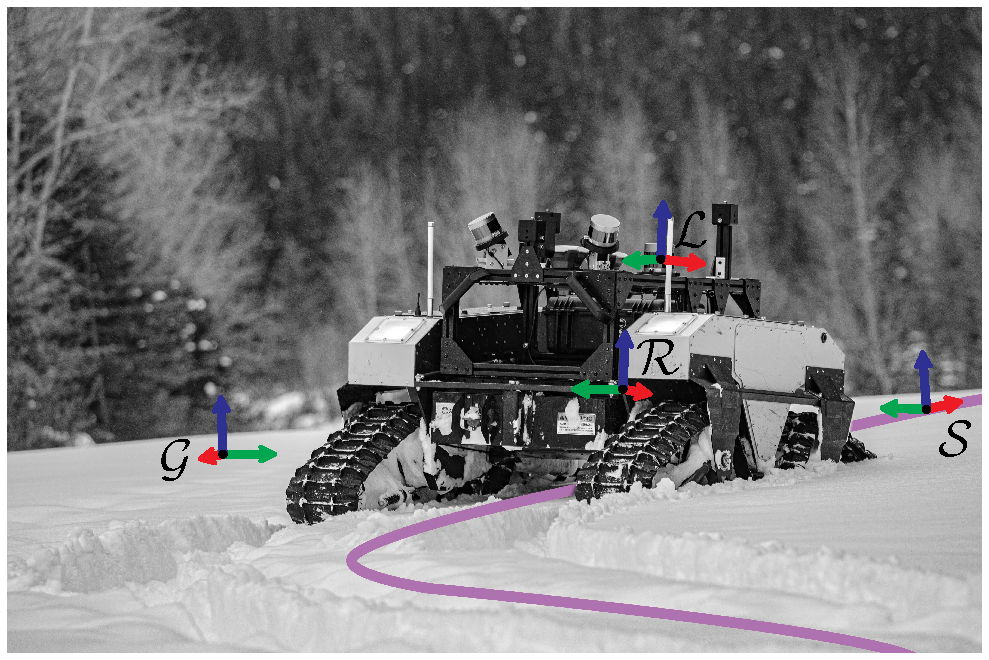
\includegraphics[width=.6\linewidth]{figs/warthog_frames/warthog_frames.pdf}
	\caption{Coordinate frames used for \ac{LTR}. The path of the robot is depicted in light blue. \todo{Describe the other frames}}
	\label{fig:ltr_frames}
\end{figure}

\subsection{Iterative closest point}
\label{ICP}

Incoming lidar scans, or reading point clouds $\readpc$ registered to a reference map, or reference point cloud $\refpc$ using the \ac{ICP} algorithm in order to localize the robot and build a map of the environment during the teach phase.
Pioneered by~\citet{Besl1992} and~\citet{Chen1991}, this algorithm iteratively matches points between two point clouds and looks for a rigid transform minimizing the distance between each matched points.
The first data processing step in our implementation is to apply input filters to $\readpc$ in order to decrease computation time and remove outlier points.
We apply two input filters to $\readpc$ : Random sub-sampling $\readpc$ and removing points that are located within pre-defined bounding boxes to remove points corresponding to the robot's body and bystanders walking behind the robot.
In our implementation, we know that $\readpc$ is observed in the lidar frame $\lidarf$ and that $\refpc$ is defined in the map frame $\mapf$.
Thus, the \ac{ICP} algorithm estimates the transform $_{\lidarf}^{\mapf}\bm{T}$ by minimizing an error function $\text{error}(\readpc, \refpc)$:

\begin{equation}
	_{\lidarf}^{\mapf}\bm{\hat{T}} = \argmin_{\bm T} (\text{error} \left(\readpc, \refpc, _{\lidarf}^{\mapf}\bm{\check{T}} \right))
\end{equation}

where $_{\lidarf}^{\mapf}\bm{\check{T}}$ is the prior transformation, estimated via the \ac{IMU} and wheel odometry.
In order to compute the error function, we associate points between $\readpc$ and $\refpc$.
This association is the done by finding the closest points in $\refpc$ for each point in $\readpc$, thus multiple points of $\refpc$ can be associated to each point of $\readpc$.
In order to accelerate this step, nearest neighbour search is done via the use of a kd-tree, as proposed by~\citet{Elseberg2012}.
In addition, binary weights are added to each point match in order to remove the outlier matches from the error function.
%Formally, let $\match = \text{match}(\readpc, \refpc) = \{(\bm p, \bm q) : \bm p \in \readpc, \bm q \in \refpc \}$ be the set of matches between $\readpc$ and $\refpc$ and $\weight = \text{outlier}(\readpc, \refpc) = \{w(\bm p, \bm q) : \forall(\bm p, \bm q) \in \match\}$ be the weights associated to these matches.
Formally, let $\match = \text{match}(\readpc, \refpc) = \{(\bm p, \bm q) : \bm p \in \readpc, \bm q \in \refpc \}$ be the set of matches between $\readpc$ and $\refpc$ and $\weight = \text{outlier}(\readpc, \refpc) = \{w(\bm p, \bm q) : (\bm p, \bm q) \in \match\}$ be the weights associated to these matches.
Our system uses point-to-plane error, which can be computed as follows

\begin{equation}
	\text{error}(\readpc, \refpc) = \sum_{k=1}^{K} w(\bm p_k, \bm q_k) \lVert (\bm p_k - \bm q_k) \cdot \bm n_k \rVert_2
\end{equation}

where $K$ is the number of matches in $\match$ and $\lVert \cdot \rVert_2$ is the L2 norm.
$\bm n_k$ is the normal vector around the 3D point $\bm q_k$ in $\refpc$, which needs to be computed prior to the \ac{ICP} algorithm.
This error can be iteratively minimized by recomputing $\match$ and $\weight$ at each iteration.
For more details, please refer to~\citep{Pomerleau2015}.
The resulting transform \transform{\lidarf}{\mapf} can be used to express the 3D robot pose in $\mapf$ by chaining \transform{\lidarf}{\mapf} \transform{\robotf}{\lidarf} since the latter is known through calibration.
An overview of the \ac{ICP} pipeline is shown in~\autoref{fig:icp_pipeline}.
Our implementation is strongly based on the \texttt{libpointmatcher}\footnote{\url{https://github.com/ethz-asl/libpointmatcher}}~\citep{Pomerleau2013}.
The parameters that were used on our system are detailed in~\autoref{tab:icp_params}.

%% Need to write on point cloud preprocessing, matching, minimization (point-to-plane) and post-processing (might be added to mapping).

\begin{figure} [htpb]
	\centering
	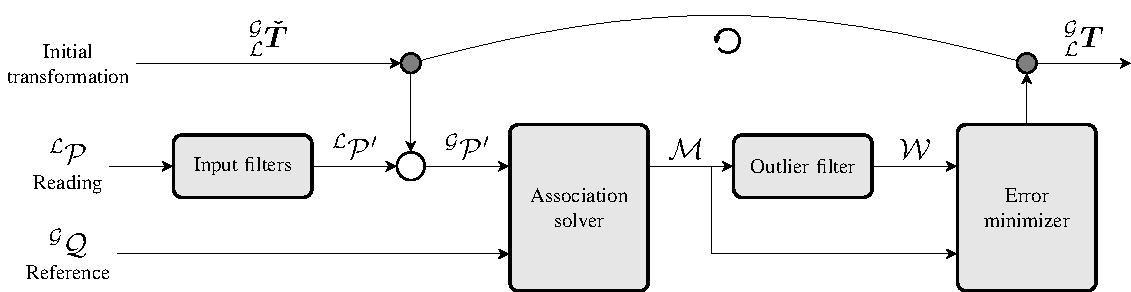
\includegraphics[width=\linewidth]{figs/icp_pipeline/icp_pipeline.pdf}
	\caption{ICP pipeline}
	\label{fig:icp_pipeline}
\end{figure}


\begin{table}[htpb]
	\caption{\ac{ICP} parameters}
	\begin{center}
		\begin{tabular}{c c c c} \toprule
			% after \\: \hline or \cline{col1-col2} \cline{col3-col4} ...
			ICP block      & Function                          & Parameters            &                       \\
			\midrule
			Input filters  & BoundingBoxDataPointsFilter       & xMin: -1.5            & xMax: 0.5             \\
			               &                                   & yMin: -1              & yMax: 1               \\
			               &                                   & zMin: -1              & zMax: 0.5             \\
			               &                                   & removeInside: 1                               \\
			               & BoundingBoxDataPointsFilter       & xMin: -10             & xMax: -1.5            \\
			               &                                   & yMin: -2.5            & yMax: 2.5             \\
			               &                                   & zMin: -1              & zMax: 1               \\
			               &                                   & removeInside: 1                               \\
			               & RandomSamplingDataPointsFilter    & prob: 0.7             &                       \\
			\midrule
			Matcher        & KDTreeMatcher                     & knn: 7                & maxDist: 2.0          \\
			               &                                   & epsilon: 1                                    \\
			\midrule
			Outlier filter & TrimmedDistOutlierFilter          & ratio: 0.7            &                       \\
			\midrule
			Cost function  & PointToPlaneErrorMinimizer        & force4DOF: 1          &                       \\
			\midrule
			Transformation & DifferentialTransformationChecker & minDiffRotErr: 0.001  & minDiffTransErr: 0.01 \\
			checkers       &                                   & smoothLength: 2                               \\
			               & CounterTransformationChecker      & maxIterationCount: 40                         \\
			\bottomrule
		\end{tabular}
	\end{center}
	\label{tab:icp_params}
\end{table}

\subsubsection{\ac{IMU} and wheel odometry and point cloud de-skewing}
\label{sec:imu_wheel_odom}
%% Move before ICP
%% Skewed PC is inverse hat

As specified above, the \ac{ICP} algorithm requires high-frequency odometry to produce a prior estimate $_{\lidarf}^{\mapf}\bm{\check{T}}$.
This estimate is produced by estimating the robot displacement between lidar scans.
Robot orientation is estimated using the Madwick filter\footnote{\url{https://github.com/bjohnsonfl/Madgwick_Filter}}~\citep{Madgwick2011} based on gyroscope and accelerometer measurements.
Linear displacement is estimated through vehicle body velocity commands.
Each command is propagated with the robot orientation between scans, yielding $_{\lidarf}^{\mapf}\bm{\check{T}}$ at a frequency of \SI{100}{Hz}.
The "force4DOF" parameter is enabled, meaning that the prior "roll" and "pitch" angle are assumed to be exact during the \ac{ICP} minimization.
In addition, it should be noted that lidar sensors typically make the assumption that the lidar frame $\lidarf$ is static during each scan, which is incorrect when the lidar sensors is subject to motion, yielding a skewed reading point cloud $\skreadpc$.
Hence, a point cloud de-skewing approach was added to our system.
First proposed by~\citet{Bosse2009}, such algorithms use the the high-frequency odometry to correct the location of each point before registration.
Following the same idea, our high-frequency odometry is used to estimate the de-skewed point cloud $\readpc$, which is the one that is used in the \ac{ICP} algorithm.


\subsection{Teach phase}
\label{sec:teach_phase}

During the teach phase, the robot is driven along a specific path by a human operator, while all sensors are used to collect data.
The \ac{ICP} algorithm is used to solve the \ac{SLAM} problem in real time, hence incoming reading point clouds $\readpc$ are registered to the reference point cloud $\refpc$ and then appended to the latter, effectively building a map.
The other output of the \ac{ICP} algorithm, the transform that allows to register the reading point cloud to the reference point cloud \transform{\lidarf}{\mapf} represents the pose of the robot $\bm x$. %JL: hard to read, simplifies sentence
By logging all robot poses, we build a reference trajectory $\reftraj$. %JL: x is a pose, but x_ref is a set(or function) of poses?  Update: ok it seems to be standard in MPC for instance. I guess just say clearly what is x_ref, like x_ref = {x_i}_i\in[0,N-1]?
The teach pipeline is illustrated in~\autoref{fig:teach_pipeline}.

\begin{figure} [htpb]
	\centering
	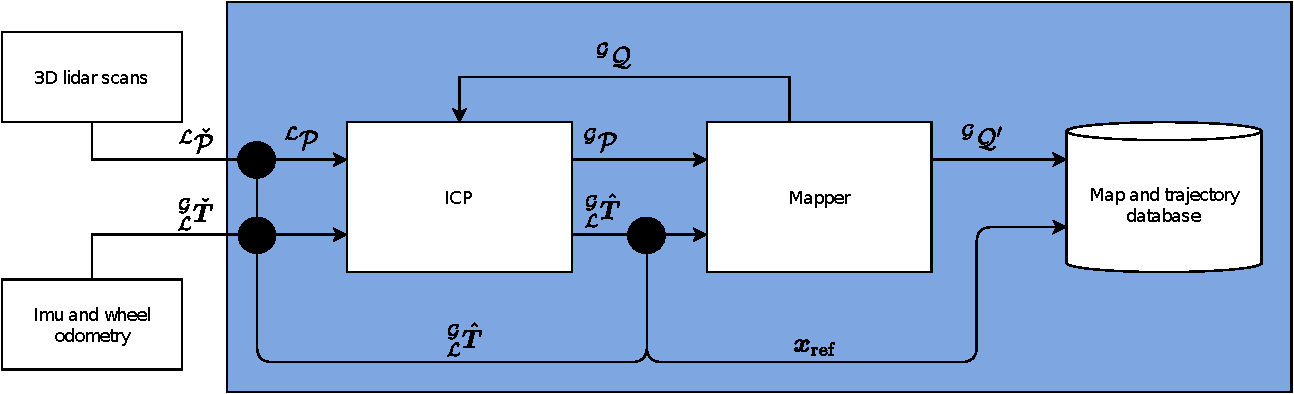
\includegraphics[height=1.8in]{figs/teach_pipeline/teach_pipeline.pdf}
	\caption{Teach phase pipeline}
	\label{fig:teach_pipeline}
\end{figure}

\subsubsection{Large-scale mapping}
\label{sec:tiled_map}

When a lidar scan, or input point cloud, $\readpc$ is acquired, it is fed to the mapping algorithm, along with the estimated lidar pose $_{\robotf}^{\mapf}\bm{\check{T}}$. %JL: too much ','
The estimated pose is provided by the odometry system decribed in~\autoref{sec:imu_wheel_odom}.
The input point cloud  $\readpc$ is first cropped to the user-defined lidar maximum range $r$. %JL: I would always define in which realm the variable lives in, but in this case it's pretty straightforward, but I'd do it anyway ! \mathbb{R}_{>0} in this case
This parameter allows to take only a portion of $\readpc$ into account when computational power is limited.
The cropped input point cloud is then registered, following the algorithm described in~\autoref{sec:ICP}, and merged into the map.
This step allows robot localization in the map and keeps the latter up to date when new portions of the environment are explored.
In order to keep a reasonable map point density, a point is only appended to the map if its distance to an existing point is above the user-defined minimal distance between two points.
After merging the input point cloud into the map, some post filters are applied to the resulting point cloud.
The first consists of computing the surface normals for all points in order to allow point-to-plane minimization.
The second one is used to filter out dynamic points, following what was proposed by~\citet{Pomerleau2014}.
This filtered point cloud then becomes the map $\refpc$ for the next iteration of the mapping algorithm.

\begin{SCfigure}
	\centering
	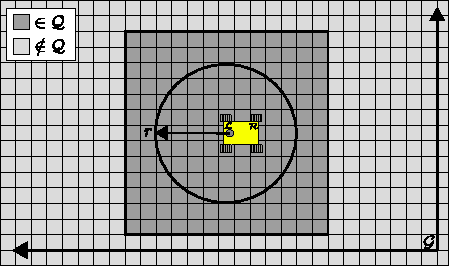
\includegraphics[height=1.8in]{figs/tiled_mapping/tiled_mapping.pdf}
	\caption{Our large-scale mapping concept illustrated.
		In green are the voxels within sensor range $r$, which constitute $\refpc$.
		In red are the voxels out of sensor range $r$, which are stored on disk.
		Voxel size is represented as $v_s$.}
	%% Mention not to scale, 2D top view
	\label{fig:tiled_map}
\end{SCfigure}

In order to save some computational power, the map is divided into voxels and only those which are inside or near the user-defined lidar maximum range are comprised in $\refpc$.
The dimension of voxels is defined as $v_s$, in meters. %same, v_s is a real positive number
Each voxel is given an integer 3D coordinate $\begin{bmatrix} v_{x}, v_{y}, v_{z} \end{bmatrix}^T \in \mathcal{Z}^3$ computed as follows:
\begin{equation*}
	\begin{bmatrix} v_{x}, v_{y}, v_{z} \end{bmatrix}^T = \floor(^{\mapf}\bm{v_o} / v_s),
\end{equation*}
where $\floor$ is a function that only keeps the integer part of the elements of a real-valued vector and $^{\mapf}\bm{v_o}$ is the position in the map frame of the origin of the voxel, which is located in its back lower left corner.
The map voxels which are farther from the robot are saved on disk for later in case they are back again near the sensor range.
When a voxel is saved on disk, it is saved in a file named: cell\_$v_x$\_$v_y$\_$v_z$.
The sum of all the voxels constitute the global map $\refpc'$, we can therefore state that $\refpc \subseteq \refpc'$. %sum or aggregation ? 'Sum of voxels' might be confusing
%A video-game-inspired algorithm is used to manage which voxels are loaded and unloaded from $\refpc'$ depending on the robot position in the map \transform{\robotf}{\mapf}. %Interesting, but miss a citation to the video-game algorithm! Otherwise there is little information in this sentence

This map segmentation technique allows us to map and localize in real time in arbitrarily large environments.
The different mapping parameters we used are listed in~\autoref{tab:mapping_params}.

%% Variables for local vs. global Q

\begin{table}[htpb]
	\caption{Mapping parameters}
	\begin{center}
		\begin{tabular}{c c c} \toprule
			Mapping block & Function                      & Parameter                    \\
			\midrule
			General       &                               & sensor\_max\_range = 80      \\
			              &                               & min\_dist\_new\_point = 0.1  \\
			              &                               & voxel\_size = 20             \\
			\midrule
			Post filters  & SurfaceNormalDataPointsFilter & knn: 15                      \\
			              & CutAtDescriptorThreshold      & descName: probabilityDynamic \\
			              &                               & useLargerThan: 1             \\
			              &                               & threshold: 0.8               \\
			\bottomrule
		\end{tabular}
	\end{center}
	\label{tab:mapping_params}
\end{table}

\subsection{Repeat phase}
\label{sec:repeat_phase}

During the repeat phase, the corresponding global map $\refpc'$ and reference trajectories $\reftraj$ are first loaded and voxels are re-built.
In this phase, no points are appended, meaning that the \ac{ICP} algorithm is only used to localize the robot.
The estimated pose of the robot \transform{\robotf}{\mapf} is then subsampled as a planar pose $\poseplane$, and then used by a path following algorithm to compute system commands $\bm u$ for the \ac{UGV} to track $\reftraj$.
Similarly as explained in~\autoref{sec:tiled_map}, only the local map $\refpc$ within sensor range $r$ is taken into account by the \ac{ICP} algorithm.
No obstacle detection feature was implemented on the system.
The repeat pipeline is shown in~\autoref{fig:repeat_pipeline}.

\begin{figure} [htpb]
	\centering
	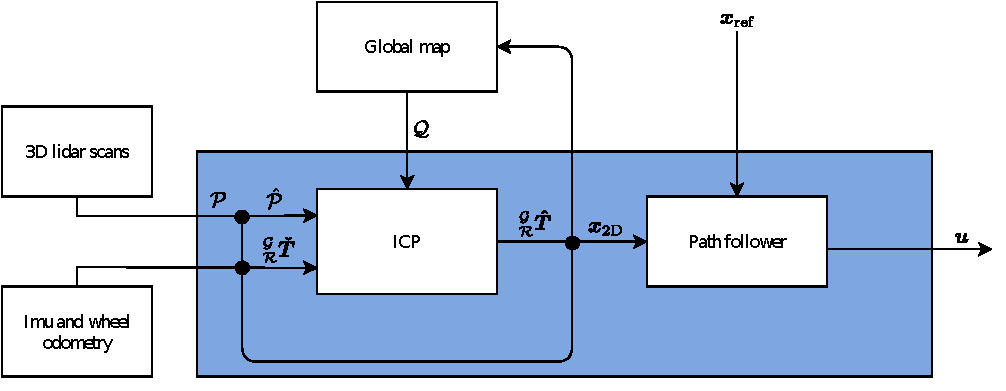
\includegraphics[height=1.8in]{figs/repeat_pipeline/repeat_pipeline.pdf}
	\caption{Repeat phase pipeline}
	\label{fig:repeat_pipeline}
\end{figure}

\subsubsection{Path following}
\label{sec:orthexp}

%% Review Frenet-Serret frame formulation from Huskic 2019

Once the robot is localized within the environment and the reference trajectory is defined, this information is used as input to a simple path following controller in order to complete the repeat pipeline.
The output of the path-following algorithm is the commanded longitudinal and angular velocities, defined in the vector $\bm u = [v_x, \omega]$.
For our implementation, we selected a simple \ac{ORTHEXP} controller.
Originally proposed by~\citet{Mojaev2004} for differential-drive mobile robots, this controller allows path tracking with a feedback loop on robot localization.
This controller was later adapted for omnidirectional mobile robots by~\citet{Li2007} and for dribbling control for soccer robots.
More recently,~\citet{Huskic2017} improved the algorithm's path following performance through heuristic linear velocity control.
To implement this controller, we used the open-source \ac{GeRoNa}\footnote{\url{https://github.com/cogsys-tuebingen/gerona}} library, created by~\citet{Huskic2019}.

%Knowing the robot's 2D pose $\poseplane$ and reference trajectory $\reftraj$, it is possible to compute the orthogonal projection $\bm P$ of the robot on the reference path.
A Frenet-Serret frame $\pathf$ is defined within the map frame with its origin corresponding to the orthogonal projection of the robot on the reference pat.
For the Frenet-Serret frame, abscissa $\bm x_t$ and ordinate $\bm x_n$ are unit tangent and unit normal vectors respectively.
The orthogonal distance from the origin of the robot frame $\robotf$ and the Frenet-Serret frame $\pathf$ along the $\bm x_n$ axis is denoted with $x_n$ and the tangential distance with $x_t$.
The tangential angle of the Frenet-Serret frame $\pathf$ with respect to the map frame $\mapf$ is defined as $\theta_t$.
The angle of robot frame $\robotf$'s $\bm x$ axis with respect to the map frame $\mapf$ is defined $\theta_r$. %JL robot frame R's -> hard to read
If we denote $x_{n_o}$ as the distance between the origin of the robot frame $\robotf$ and the origin of the path frame $\pathf$, it is possible to define the following exponential law as
\begin{equation}
	\label{eq:exp_law}
	x_n = x_{n_o} e^{-k x_t},
\end{equation}
where $k$ is a positive constant that allows to regulate the convergence speed of the robot to the path.
Next, the exponential function's tangent angle with the map frame $\phi_e$ can be computed as follows:
\begin{equation}
	\label{eq:exp_angle}
	\phi_e = \arctan(-k x_n).
\end{equation}

The angular velocity command can then be computed as %JL: remove some "as follows" before the equation and added punctuation
\begin{equation}
	\label{eq:exp_PD}
	\omega = K_h (\phi_e + \theta_e),
\end{equation}
where $\theta_e$ is the error between the robot angle $\theta_r$ and the path frame angle $\theta_t$.
The $K_h$ parameter is a gain on commanded angular velocity that was added after we empirically observed that the robot stabilizes at an angular velocity significantly lower than the commanded angular velocity, based on \ac{IMU} measurements.
A summary of the geometrical representation of the variables affecting the angular velocity command is shown in~\autoref{fig:diff_orthexp}.

\begin{SCfigure}
	\centering
	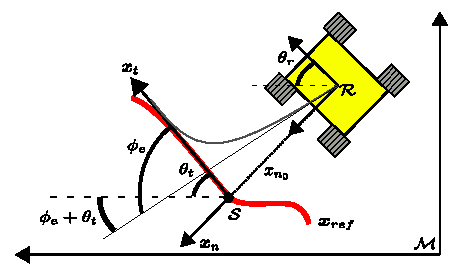
\includegraphics[height=1.6in]{figs/path_follower/orthexp.pdf}
	\caption{Main components of the \ac{ORTHEXP} path following algorithm used in this work.
		In red is the reference trajectory.}
	\label{fig:diff_orthexp}
\end{SCfigure}

In the \ac{GeRoNa} library, commanded longitudinal velocity $v_x$ can be computed based on multiple factors such as upcoming path curvature, current vehicle angular velocity, proximity of obstacles and distance from the end goal.
Due to \ac{ICP} localization noise in the teach phase, the upcoming path curvature would sometimes peak causing the robot to stop on the spot, we therefore removed this factor.
Current vehicle angular velocity has also been removed from the equation to simplify controller parameter tuning.
In our system, no obstacle detection feature is included, meaning that the proximity of obstacles cannot be used as a factor to compute linear velocity.
It is only the distance from the end goal that was used in order to prevent the robot from finishing its course abruptly.
Thus, the commanded linear velocity $v_x$ is computed as
\begin{equation}
	\label{eq:exp_lin_vel}
	v_x = v_n \exp\left(-\left(\frac{K_g}{d_g}\right)\right),
\end{equation}
where $v_n$ is the target vehicle velocity and $d_g$ is the distance between the robot's pose and the last pose of the final reference trajectory pose.
At each time step, a new exponential function and command $\bm u$ are computed using the control laws shown in~\autoref{eq:exp_PD} and~\autoref{eq:exp_lin_vel}, using the robot's 2D pose $\poseplane$ and reference trajectory $\reftraj$ as input.
The parameters for the \ac{ORTHEXP} controller were tuned empirically by having the robot repeating arbitrary short trajectories and minimizing error, these parameters are detailed in~\autoref{tab:orthexp_params}.


\begin{table}[htpb]
	\caption{\ac{ORTHEXP} controller parameters} \label{tab:orthexp_params}
	\begin{center}
		\begin{tabular}{c c c c c c} \toprule
			% after \\: \hline or \cline{col1-col2} \cline{col3-col4} ...
			General            &              & Angular velocity     &                 & Linear velocity                 \\
			\midrule
			Waypoint tolerance & \SI{1.0}{m}  & $k$                  & 0.4             & $K_g$           & 0.5           \\
			Goal tolerance     & \SI{0.15}{m} & $K_g$                & 0.5             & $v_n$           & \SI{1.5}{m/s} \\
			                   &              & $K_h$                & 3.0             & $v_{min}$       & \SI{0.5}{m/s} \\
			                   &              & Max angular velocity & \SI{1.0}{rad/s} & $v_{max}$       & \SI{1.5}{m/s} \\
			\bottomrule
		\end{tabular}
	\end{center}
\end{table}

\subsection{Hardware description}
\label{sec:hardware}

Our system was deployed on a Clearpath Robotics Warthog \ac{UGV}.
The Warthog is a \ac{SSMR} using two drive units located on each side of its chassis.
For \acp{SSMR}, steering is done by sending rotating the wheels on each side of the vehicle at different velocities to creating a skidding effect, effectively turning the vehicle.
Vehicle motion control is done through a sub-servo system allowing to control each side's wheel velocity through Sevcon Gen4 drives and aformentionned wheel encoders signal.
A kinematic linear mapping between wheel velocities and body velocities allows to send body-velocity commands directly to the platform.
Finally, the platform is symmetrical, meaning that it is able to drive along each path both forwards and backwards.
The Warthog is mounted on CAMSO ATV T4S tracks in order to maximize mobility.
The Warthog is also equipped with a differential suspension, maximizing track or wheel traction when navigating steep terrain.
Our vehicle is also equipped with a standard sensor suite for autonomous navigation.
In order to enable the \ac{LTR} framework, a Robosense RS-32 3D lidar is mounted in front of the robot, for this work, it is the only lidar used for localization.
This lidar has a \SI{200}{m} detection range and produces about \SI{640000}{} points per second.
3 Hall effect sensors are added to each motor to provide wheel odometry for the robot.
Finally, an XSens MTi-10 \ac{IMU} provides angular velocity and body linear acceleration measurements.
Additional sensors used for recording in this work include a Dalsa C1920 camera and two Emlid Reach-RS+ \ac {RTK} \ac{GPS} receivers.
Two Robosense RS-16 lidars were added to the rear of the platform to collect measurements on tree canopy but no data was recorded through those sensors.
All technical specifications for the platform are given in~\autoref{fig:warthog}.

\begin{figure} [h!]
	\centering
	\begin{minipage}[b]{1.0\linewidth}
		\centering
		\begin{tabular}[b]{l r} \toprule
			\textbf{Physical}         &                                      \\
			% after \\: \hline or \cline{col1-col2} \cline{col3-col4} ...
			Mass                      & \SI{590}{kg}                         \\
			Footprint                 & 2.13 x 1.52 m                        \\
			Top speed                 & \SI{18}{km/h}                        \\
			Steering geometry         & Skid-steering                        \\
			Locomotion                & CAMSO ATV T4S Tracks                 \\
			Suspension                & Geometric Passive Articulation       \\
			\midrule
			\textbf{Electrical}                                              \\
			Battery type              & AGM sealed lead acid                 \\
			Batteries nominal voltage & \SI{48}{V}                           \\
			Motor controllers         & Sevcon Gen4                          \\
			\midrule
			\textbf{Sensors}                                                 \\
			Front lidar               & Robosense RS-32 (\SI{10}{Hz})        \\
			\ac{IMU}                  & XSens MTi-10 (\SI{100}{Hz})          \\
			Wheel encoders            & 3 x hall effect sensors (\SI{4}{Hz}) \\
			Camera                    & Dalsa C1920 (\SI{8}{Hz})             \\
			\ac{GPS}                  & Emlid Reach-RS+ (\SI{5}{Hz})         \\
			\midrule
			\textbf{Computing}                                               \\
			Computer                  & Acrosser AIV-Q170V1FL                \\
			CPU                       & i7-6700 TE                           \\
			RAM                                                              \\
			Memory                                                           \\
			\bottomrule
		\end{tabular}
		\qquad
		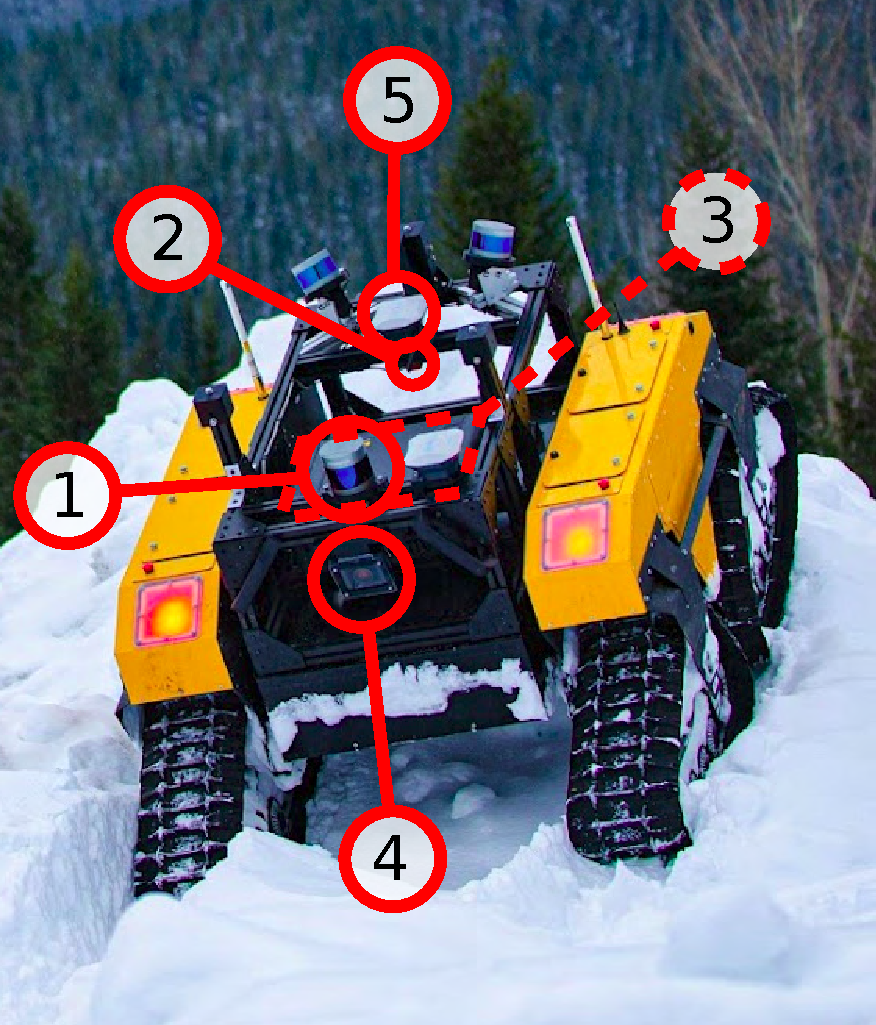
\includegraphics[height=3in]{figs/warthog_hardware.pdf}
	\end{minipage}
	\caption{The experimental setup for \ac{LTR} on our Clearpath Robotics Warthog \ac{UGV}: (1) Robosense RS-32 lidar, (2) XSens MTi-10 \ac{IMU}, (3) Acrosser AIV-Q170V1FL computer, (4) Dalsa C1920 color camera, (5) 2 Emlid Reach-RS+ \ac{GPS} antennas. \todo{why dotted line}}
	\label{fig:warthog}
\end{figure}
